\documentclass{beamer}
\usetheme[pageofpages=de,% String used between the current page and the
                         % total page count.
          bullet=circle,% Use circles instead of squares for bullets.
          titleline=true,% Show a line below the frame title.
          alternativetitlepage=true,% Use the fancy title page.
          titlepagelogo=../img/fse_ministerio_ancho_texto.png%,% Logo for the first page.
	  %watermark=junta_girado,
          %watermarkheight=75px,% Height of the watermark.
          %watermarkheightmult=4,% The watermark image is 4 times bigger
                                % than watermarkheight.
          ]{Torino}

\usepackage[spanish]{babel} % Para separar correctamente las palabras
\usepackage[utf8]{inputenc} % Este paquete permite poner acentos y eñes usando codificación utf-8

\usepackage{color}

\author{IES Gonzalo Nazareno\\
IES Los Albares\\
IES La Campiña\\
IES Ingeniero de la Cierva\\
\vspace{.5cm}

\includegraphics[width=0.2\textwidth]{cc_by_sa.png}}
\title{OpenStack nova CLI}
\institute{Proyecto de Innovación\\ {\color{white} .\\} \emph{Implantación y puesta a punto de la infraestructura de un cloud computing privado para el despliegue de servicios en la nube}} 


\begin{document}
\begin{frame}[t,plain]
\titlepage
\end{frame}

\begin{frame}
  \frametitle{Utilización de nova CLI}
  \begin{itemize}
  \item De forma análoga a lo presentado en \textit{Introducción a OpenStack
      Horizon}, vamos a realizar las acciones básicas de manejo de instancias,
    pero utilizando en este caso la aplicación \textit{nova} desde línea de
    comandos.
  \item Es necesario instalar en el equipo el paquete \textit{python-novaclient}
  \item Los pasos a seguir son:
    \begin{itemize}
    \item Autenticar el usuario
    \item Crear y manejar un par de claves RSA
    \item Realizar ajustes del Grupo de Seguridad
    \item Listar las imágenes disponibles
    \item Lanzar una instancia
    \item Asociar una IP flotante
    \item Acceder a la instancia
    \item Realizar algunas acciones sobre la instancia
    \end{itemize}
  \end{itemize}
\end{frame}

\begin{frame}[fragile]
  \frametitle{Autenticación}
  Es necesario definir varias variables de entorno para poder utilizar
  \textit{nova}, la forma más sencilla es obtener el fichero openrc.sh de
  Horizon:
  \begin{itemize}
  \item \textit{Settings $>$ OpenStack Credentials $>$ Download RC file}
  \end{itemize}
\begin{verbatim}
usuario@jupiter:~$ source openrc.sh 
Please enter your OpenStack Password:
\end{verbatim}
  \begin{columns}
    \column{.5\textwidth}
    \begin{itemize}
    \item Con lo que se definen en la sesión las variables de entorno:
      \begin{itemize}
      \item OS\_AUTH\_URL
      \item OS\_TENANT\_ID
      \item OS\_TENANT\_NAME
      \item OS\_USERNAME
      \item OS\_PASSWORD
      \end{itemize}
    \end{itemize}
    \column{.5\textwidth}
    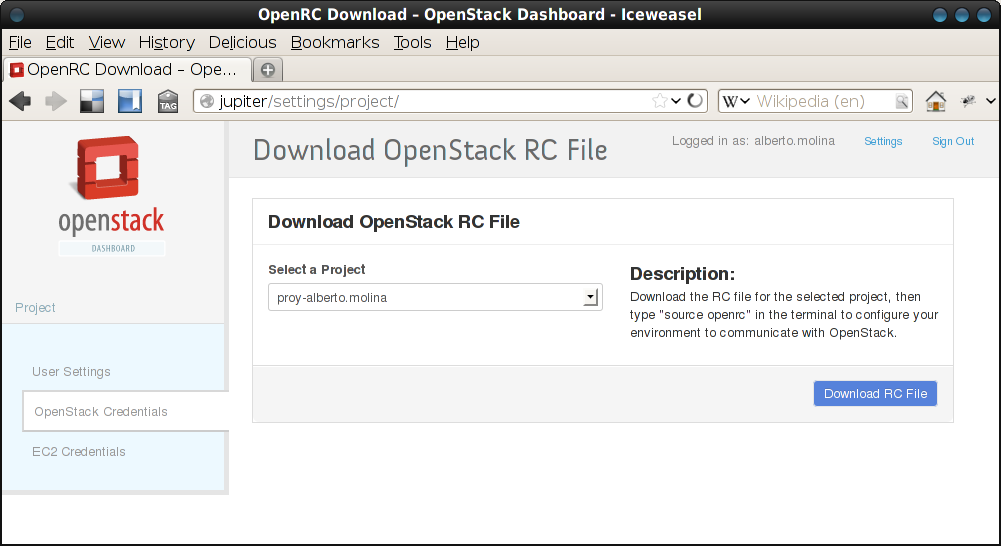
\includegraphics[width=\columnwidth]{../img/nova1.png}
  \end{columns}
\end{frame}
\begin{frame}
  \frametitle{Pares de clave RSA}
  \begin{itemize}
  \item Creamos un par de claves RSA pública/privada en nuestro equipo:
  \end{itemize}
\begin{verbatim}
$ cd ~/.ssh
$ ssh-keygen
\end{verbatim}
\end{frame}

\end{document}

